\documentclass[11pt]{article}
\usepackage[margin=0.85in]{geometry}
\usepackage{amsmath,amssymb,graphicx,booktabs,longtable,array,xcolor,hyperref,fancyhdr,microtype}
\definecolor{ink}{HTML}{164D70}
\hypersetup{colorlinks=true,linkcolor=ink,urlcolor=ink,citecolor=ink}
\setlength{\parindent}{0pt}\setlength{\parskip}{6pt}
\setlength{\headheight}{15pt}
\pagestyle{fancy}\fancyhf{}\fancyhead[L]{\small Computational neurophysiology: frozen suite}
\fancyhead[R]{\small 18 October 2026}\fancyfoot[C]{\thepage}
\setcounter{topnumber}{2}\setcounter{bottomnumber}{2}
\renewcommand{\floatpagefraction}{0.65}
\newcommand{\R}{\mathbb{R}}
\emergencystretch=1em
\usepackage{capt-of}
\begin{document}

\title{Biological experiments, theory and the 19-task observer}
\author{Literature-grounded analysis of the frozen previous model}
\date{18 October 2026}\maketitle
This companion connects each task to multiple human or animal experiments, explains the proposed computation, and compares that proposal with the model's behavior, attention, state interventions and decoding results. Each chapter ends with a discriminating experiment motivated by the actual agreement or difference. The full task papers contain the complete psychometrics, time-resolved attention figures, population analyses and intervention sweeps.

The computational subject is the previous architecture at update 204,289. Its final saved state at 220,637 is a separate robustness comparison in the task papers. The fresh spatial-memory-query cloud experiment is a separate subject. The present comparison uses 248,352 completed model evaluations and adds descriptive reanalyses of existing motion-duration and recognition trials, with zero new model forwards.

\clearpage\setcounter{tocdepth}{1}\tableofcontents\clearpage
\section{A common framework for comparing the experiments}
\subsection{From sensory content to selection, memory and report}
Four questions organize the evidence. What information reaches the visual representation? Which information receives priority? What remains available after the input disappears? Which available information actually controls the report? A successful answer to one question does not settle the others. The static object-search result makes this separation especially concrete: a decoded memory can support a strong external matcher while the trained agent chooses poorly. Motion search provides a successful comparison in the same broad architecture.

Each model site contains a vector of visual attributes. Spatial attention assigns a coefficient to that vector. If $v_s$ is the vector at site $s$ and $\alpha_s$ its attention weight, a selected summary has the form $u=\sum_s\alpha_s v_s$. Here $u$ is the pooled representation, the sum runs over spatial sites, and all components of a selected site's vector contribute through the same spatial coefficient. This is a concrete shared-selection hypothesis for static and motion information. Different sensory feature transformations can feed that common selection mechanism.

\subsection{What a local attention perturbation predicts mathematically}
Let $A$ be the total attention weight inside a selected region before a uniform logit dose $\delta$. Softmax normalization gives
\[
A'=\frac{e^\delta A}{1-A+e^\delta A}.
\]
Positive $\delta$ increases the region's odds of selection and negative $\delta$ decreases them. The unperturbed regions inherit the remaining total weight. This redistribution is a property of the intervention. A behavioral benefit elsewhere additionally requires usable evidence and a readout that can exploit it. The VDA experiments measure those two levels separately: the map changes, but the full reciprocal behavioral benefit is absent at the tested weak strengths.

\subsection{Biased competition, normalization and dynamic memory}
Biased competition proposes that attention favors one of several represented stimuli. Divisive-normalization theory implements a related interaction between excitatory drive and pooled suppression. These ideas motivate testing target-alone and target-with-competitor responses under controlled attention. Our softmax has a shared spatial denominator; the sensory and recurrent layer-normalization operations have different roles. The physiological theory is best tested through response functions across stimulus and attention conditions, rather than through the name of a normalization operation. \cite{bio_competition,bio_normalization}

Memory theories also make different predictions about what remains stable. A persistent population pattern, a changing code with preserved information, and a reconstruction from another state can all support a later correct response. Cross-time decoding measures transfer of a fixed readout; state perturbation measures dependence at a particular moment. Combining them with content reconstruction connects representation and behavior. Dynamic prefrontal coding motivates this temporal approach. \cite{bio_stokes}

\subsection{Interpreting agreement at the right experimental level}
The chapters distinguish agreement in behavior, agreement in the represented variable, and agreement in causal dependency. A spatial logit dose is specified in model units; electrical stimulation and pharmacological inactivation act on biological tissue. Comparisons therefore focus on experimentally matched patterns: which location improves or worsens, which event is falsely reported, which content is recoverable, and when a perturbation matters. Model frame counts measure computational updates. A conversion to milliseconds requires a separate timing model.

Published biological studies are summarized from the verified primary sources listed in the references. The source ledger records whether the evidence inspected was an author abstract, figure legends or article text. The proposed follow-up experiments are explicitly separated from completed results. The chapters give multiple experimental anchors for every task and use theory to explain how those anchors constrain the computation.
\clearpage\section{From local correspondence to cardinal motion decisions}
\textbf{Scientific question.} How does a population representation of image displacement become a direction judgment?

The frozen checkpoint at update 204,289 achieved an equal-condition mean accuracy of 100.00\% across 1 native conditions (128 trials). The following comparisons use that same checkpoint and the measured interventions and population recordings in this paper.

\subsection{What the model measurements establish}
The large increase in direction decodability between appearance and fusion places an accessible direction signal upstream of the recurrent decision states. The neural-state resets produced little impairment at the native displacement strengths, and the long-window comparison state was zero. Together, these observations favor a computation in which the short-lag correspondence representation already supplies sufficient directional evidence for the downstream classifier. The correspondence bank itself uses preceding pixels; resetting a recurrent neural state leaves that causal visual history available. The weak-displacement curve supplies the more sensitive test of the front end than native ceiling performance. A spatial redistribution can also leave many informative dots available, explaining why strong direction information and small quadrant-perturbation effects can coexist.

\subsection{Britten, Shadlen, Newsome and Movshon (1992): macaque experiment}
In stochastic-motion discrimination, sensitivity of many individual MT neurons approached behavioral sensitivity when stimuli were tailored to the recorded neuron. The study compared neuronal and behavioral discrimination on the same task. \cite{bio_britten}

Our visual-to-fusion decoding increase supplies a computational counterpart to the distinction between sensory evidence and a report. A useful comparison is the entire neurometric-versus-psychometric curve as displacement weakens. Native accuracy at ceiling contributes little to that comparison. The animal experiment varied stochastic-motion strength; our existing challenge varies pixel displacement, which changes correspondence ambiguity and rasterization. These manipulate different sources of uncertainty.

\subsection{Salzman, Britten and Newsome (1990): macaque experiment}
Electrical stimulation of direction-selective MT clusters biased reported motion toward the preferred direction of the stimulated population, linking a characterized sensory code to a perceptual decision. \cite{bio_salzman}

The present quadrant intervention changes where evidence is sampled. MT microstimulation changes the balance of direction-selective evidence. A small quadrant effect in a full-field movie therefore fits distributed evidence: useful dots remain elsewhere. A closer causal experiment would identify direction-preferring fused coordinates on independent fitting trials, perturb those coordinates during weak motion, and ask whether choices shift toward the fitted preferred direction.

\subsection{Ling, Liu and Carrasco (2009): human experiment and theory}
External-noise motion experiments separated spatial from feature-based attention. Threshold-versus-noise functions supported different combinations of population gain and tuning, giving behavioral tests of attentional mechanisms. \cite{bio_ling}

The human noise manipulation provides a way to distinguish stronger evidence from rejection of irrelevant directions. Our correspondence front end already compares local image shifts; successful direction decoding can follow from that operation. Varying dot-direction noise while holding speed, contrast and dot count fixed would reveal whether the learned readout pools direction evidence robustly or depends on nearly uniform displacement.

\subsection{Theory and the model computation}
The relevant theory is population decoding. A candidate direction is supported by a pattern across channels, and a downstream computation must compare competing patterns. In this model, the fixed correspondence calculation supplies local displacement alternatives and learned fusion converts them into task-useful features. Spatial attention then determines which sites contribute. These are three distinct operations: estimate local correspondence, represent a direction, and pool it for a decision. Their separation explains why strong direction information can coexist with weak effects of redistributing attention across a uniformly informative display. The previous-frame pixel history also survives a reset of neural recurrent memory, so the reset experiment tests the added recurrent contribution after short-lag visual evidence is already available.

\subsection{Agreement, difference and scientific interpretation}
The agreement is a readable sensory code that supports accurate direction decisions. The strongest mechanistic distinction is the engineered correspondence bank preceding the learned network. Current observations support efficient use of that bank; the relation to MT becomes more specific when channel tuning and direction-selective perturbations are measured together.

\subsection{The next discriminating experiment}
Cross displacement with motion coherence and contrast, fit direction tuning on independent movies, and perturb matched versus mismatched direction populations. Predict a horizontal choice-curve shift for a directional evidence bias and a threshold change for reduced evidence reliability.

This last experiment is a proposed test; the results above are the completed frozen-model measurements.
\clearpage\section{Signed orientation comparison through recurrent visual memory}
\textbf{Scientific question.} How is the orientation of one observation retained and compared with a later observation?

The frozen checkpoint at update 204,289 achieved an equal-condition mean accuracy of 100.00\% across 1 native conditions (128 trials). The following comparisons use that same checkpoint and the measured interventions and population recordings in this paper.

\subsection{What the model measurements establish}
Orientation ordering becomes much more readable in recurrent states than in the capacity-matched appearance and fused representations. Resetting the global reference-period state produced a substantial subsequent error increase, with an additional cost from resetting spatial memory. This pattern links the final response to information carried across the two observations. Concentrating priority in a fixed quadrant also impaired performance, even though the grating occupies the full image. The relevant spatial question is therefore how the selected sample supports a stable comparison, rather than whether an isolated target object receives more attention. The combination of perturbation and decoding localizes a comparison computation more strongly than final CLS decodability alone.

\subsection{De Valois, Yund and Hepler (1982): macaque experiment}
Striate neurons exhibited a broad distribution of orientation bandwidths and both direction-selective and direction-insensitive responses. Orientation and motion selectivity were measured as tuning properties of individual cells. \cite{bio_devalois_o}

The biological measurement concerns a neuron’s response as absolute orientation changes. Our answer decoder concerns the sign of a difference between two orientations. Those quantities should be separated experimentally: first map absolute-angle tuning, then measure whether comparison information appears only after the second image. Strong late answer decoding can arise even when early features represent both angles in a distributed form.

\subsection{Harrison and Tong (2009): human experiment}
Human fMRI patterns in V1-V4 identified the remembered grating orientation during a blank delay, including cases with little sustained average activation. Information in a population pattern could persist despite low mean activity. \cite{bio_harrison}

Our recurrent-state reset costs connect the first observation to the later decision. The human result motivates decoding the retained angle itself during the intervening state. An answer label alone is insufficient before the second angle defines clockwise or counterclockwise. Testing angle reconstruction and then resetting its carrier would link represented content to comparison behavior.

\subsection{McAdams and Maunsell (1999): macaque experiment}
During an orientation attention task, V4 responses increased with attention largely through scaling of tuning curves, without a systematic change in tuning width. V1 modulation was smaller. \cite{bio_mcadams}

Concentrating priority in a quadrant harms this model’s full-field comparison. This is compatible with losing useful distributed evidence, whereas the V4 experiment measures gain for an attended stimulus. To compare them, hold the grating and response rule fixed and measure coordinate tuning with and without a spatial-priority bias. The shape of that tuning curve matters in addition to its amplitude.

\subsection{Theory and the model computation}
A natural computational account has an encoding stage, a retained reference, and a signed comparison. Because orientation repeats after 180 degrees, a stable representation uses two coordinates, cosine and sine of twice the angle. A readout comparing those coordinates can distinguish nearby rotations while respecting the wrap at 180 degrees. The existing state-reset results support a role for retained reference information: removing global or spatial memory after the reference impairs the final report. The mechanism could preserve an angle, a richer image representation, or both. The two-frame native sequence makes these hypotheses especially testable through controlled changes in phase, frequency and contrast between the observations.

\subsection{Agreement, difference and scientific interpretation}
Behavior agrees with accurate sequential orientation discrimination, and recurrent perturbation identifies a causal dependence on reference-period state. Agreement with a specific cortical tuning mechanism remains an empirical question about absolute-angle response profiles and generalization across nuisance features.

\subsection{The next discriminating experiment}
Independently randomize grating phase and contrast across the two observations. Decode the first angle before the probe and compare preferred-angle tuning across states. If a transferable orientation reference drives the task, signed judgment should survive nuisance changes that preserve the two orientations.

This last experiment is a proposed test; the results above are the completed frozen-model measurements.
\clearpage\section{Contrast comparison, spatial selection and recurrent state dependence}
\textbf{Scientific question.} Does the model compare a retained contrast signal, and does its sensitivity follow the nonlinear contrast behavior seen in vision?

The frozen checkpoint at update 204,289 achieved an equal-condition mean accuracy of 100.00\% across 1 native conditions (128 trials). The following comparisons use that same checkpoint and the measured interventions and population recordings in this paper.

\subsection{What the model measurements establish}
The fused representation already carries appreciable information about the correct interval, and recurrent populations make that information nearly fully readable. The largest reference-period memory-reset cost came from spatial memory. This connects the accurate final comparison to a retained spatial description of the first interval. Absolute contrast and the temporal image representation can each provide partial cues; the high terminal accuracy and reset effects reveal how those signals are combined in the trained observer. The subthreshold increment sweep measures the limit of that computation, while quadrant interventions test how concentrated sampling changes the reliability of the evidence being compared.

\subsection{Legge and Foley (1980): human experiment}
Human grating discrimination showed facilitation at weak masking contrasts and increased thresholds at stronger masks. A nonlinear contrast transducer, spatial filtering and pooling explained the dependence on masker strength and frequency. \cite{bio_legge}

Our increment challenge asks how small a contrast difference the observer can use. The human result asks how that threshold changes with the reference or masking contrast. Native ceiling accuracy and a single pooled increment curve cannot reveal the low-pedestal facilitation and high-pedestal masking pattern. The decisive comparison is a separate threshold curve at each pedestal, using the same spatial frequency and timing.

\subsection{Reynolds, Pasternak and Desimone (2000): macaque experiment}
Attention increased V4 responses more strongly at low than high stimulus contrast. The pattern was consistent with an increase in effective contrast, connecting attentional state with sensory sensitivity. \cite{bio_reynolds00}

The monkey measurement is a contrast-response curve of a sensory population under attention. Our manipulation changes normalized spatial routing. To compare mechanisms, record the model’s fused or recurrent response across contrast under the same attended and unattended geometry, then fit response amplitude and horizontal contrast shift separately. A behavioral improvement by itself would leave both possibilities open.

\subsection{Campbell and Robson (1968): human experiment}
Thresholds for several grating waveforms were explained by the visibility of their Fourier components. Higher harmonics became behaviorally useful when they exceeded their own thresholds, supporting frequency-selective visual mechanisms. \cite{bio_campbell}

Contrast has meaning relative to a spatial pattern. Frequency-selective detection explains why an equal numerical contrast need not be equally visible for every grating. The model has a finite raster, fixed site spacing and learned image features. Varying frequency alongside pedestal would test whether its thresholds reflect a visual filter bank or a broad image-statistic comparison.

\subsection{Theory and the model computation}
Contrast discrimination combines a sensory transducer with comparison memory. A saturating transducer can make the same physical increment produce different internal differences at different pedestals. The spatial-memory reset cost in the present task shows that the reference image leaves a behaviorally useful spatial state. The final recurrent readout can then compare a new contrast-dependent pattern with that reference. Normalization theory adds a second operation: the response to one drive depends on competing drive. Layer normalization in the recurrent unit stabilizes channel scale, while attention softmax redistributes spatial weight. Their mathematical normalization does not by itself determine a physiological contrast-response law; that law must be measured by the pedestal experiment. \cite{bio_normalization}

\subsection{Agreement, difference and scientific interpretation}
The model agrees with the broad requirement for retaining and comparing contrast-bearing evidence. The available data establish fine discrimination under the tested rendering. The characteristic pedestal dependence of human vision is the sharper biological test, and it is not determined by the present native ceiling result.

\subsection{The next discriminating experiment}
Estimate thresholds over a two-dimensional pedestal-by-increment grid, with absolute frequency controlled. Repeat under broad and concentrated attention. Fit a saturating transducer and ask whether one parameter set predicts held-out pedestals and attention conditions.

This last experiment is a proposed test; the results above are the completed frozen-model measurements.
\clearpage\section{Spatial-frequency discrimination in a shared visual architecture}
\textbf{Scientific question.} How can an observer report which of two gratings is finer, and what would establish a channel-based comparison?

The frozen checkpoint at update 204,289 achieved an equal-condition mean accuracy of 100.00\% across 1 native conditions (128 trials). The following comparisons use that same checkpoint and the measured interventions and population recordings in this paper.

\subsection{What the model measurements establish}
The answer is most clearly expressed in global recurrent memory, while both global and spatial reference-period resets impair the subsequent judgement. The results support a sequential representation of interval ordering rather than a direct interpretation of a single local edge detector. Spatial priority concentration can additionally reduce performance, consistent with the decision using evidence distributed over the grating. The octave axis makes the behavioral curve a test of relative frequency discrimination. Extending the pedestal range would determine whether the comparison remains accurate when the same relative difference is embedded in unfamiliar absolute frequencies.

\subsection{Campbell and Robson (1968): human experiment}
Thresholds for several grating waveforms were explained by the visibility of their Fourier components. Higher harmonics became behaviorally useful when they exceeded their own thresholds, supporting frequency-selective visual mechanisms. \cite{bio_campbell}

Our task compares frequencies above visibility threshold; the classic human experiment measured when components became visible. Both motivate describing image structure by scale, but successful frequency ordering does not establish the detector thresholds of separate Fourier components. Testing compound gratings would ask whether the model follows the fundamental or a more visible harmonic.

\subsection{De Valois, Albrecht and Thorell (1982): macaque experiment}
Measurements of striate neurons revealed many narrow spatial-frequency bandwidths and a wide range of preferred frequencies at a given eccentricity, supporting multiple spatial-frequency channels. \cite{bio_devalois_f}

A biological channel account predicts different preferred frequencies across a population. The model’s appearance features and fixed crops offer candidate populations to inspect. Map each coordinate’s response across frequency, phase and orientation, then test whether a decoder trained on some phases generalizes to new phases. This would identify a scale representation rather than a particular stripe pattern.

\subsection{Regan and Beverley (1983): human experiment}
Adaptation altered frequency-discrimination and grating-detection thresholds differently. The dissociation supported a distinction between detecting channel activity and comparing relative responses across overlapping channels. \cite{bio_regan}

Detection and discrimination can change differently because the operations read different aspects of channel activity. Our recurrent reset costs identify a sequential comparison dependency. A model adaptation experiment would need an explicit adaptation process or a controlled preceding stimulus sequence; merely lowering the contrast of a test image would address visibility instead of the historical adaptation manipulation.

\subsection{Theory and the model computation}
On a logarithmic frequency axis, a fixed octave increment means a fixed ratio between frequencies. A population of overlapping scale-sensitive channels can encode frequency by the relative distribution of its activity; a retained distribution from the first image can then be compared with the second. This is a plausible account of the strong final global-memory answer code and the costs of resetting either reference-period state. Concentrating attention can reduce the number of visible cycles sampled and make that estimate less stable. The 100-pixel image also creates a concrete sampling limit: the highest frequencies approach the raster’s resolution and can change appearance sharply with phase. Separating scale sensitivity from aliasing is therefore essential to the interpretation.

\subsection{Agreement, difference and scientific interpretation}
The agreement lies in scale-dependent visual evidence followed by a memory-dependent ordering judgment. The missing biological signature is a measured distribution of frequency tuning and its relation to thresholds across absolute frequencies. The present decoder results localize usable information without identifying the receptive-field basis that carries it.

\subsection{The next discriminating experiment}
Sweep reference frequency over a wider range while holding octave differences fixed. Include independently randomized phase and compound gratings. Relate errors to measured channel tuning and to the number of cycles inside attended crops.

This last experiment is a proposed test; the results above are the completed frozen-model measurements.
\clearpage\section{Chromatic interval comparison under shared spatial priority}
\textbf{Scientific question.} How does a shared spatial-selection network use color information when its motion calculation is grayscale?

The frozen checkpoint at update 204,289 achieved an equal-condition mean accuracy of 100.00\% across 1 native conditions (128 trials). The following comparisons use that same checkpoint and the measured interventions and population recordings in this paper.

\subsection{What the model measurements establish}
Accurate chromatic comparison survives in an architecture whose motion correspondence calculation uses grayscale input. The measured behavior is therefore supported by the color-bearing appearance and local-statistic channels together with recurrent processing. Both global and spatial reference-period resets have substantial effects, and the final answer is strongly readable in those recurrent populations. This provides a static-feature case for a shared spatial-selection architecture: the same priority distribution participates in a computation whose defining information is chromatic. A small effect of one quadrant manipulation can coexist with strong memory dependence when useful color evidence is present throughout the field.

\subsection{Derrington, Krauskopf and Lennie (1984): macaque experiment}
Color-space null measurements characterized how LGN neurons combine cone signals. The results exposed opponent chromatic mechanisms and separated chromatic from luminance-dependent response directions. \cite{bio_derrington}

The model receives RGB image coordinates, whereas the LGN study used cone-derived color coordinates. RGB increments have no direct physiological unit without a display spectrum and cone calibration. The useful comparison is structural: does the learned representation separate changes along independent color directions, and can those signals be selected and retained for a decision?

\subsection{Lennie, Krauskopf and Sclar (1990): macaque experiment}
V1 neurons responded to combinations of chromatic and luminance modulation. Their distribution of preferred color directions differed from the more distinctly grouped LGN mechanisms, showing a cortical transformation of cone-derived signals. \cite{bio_lennie}

Cortical transformations can mix chromatic and luminance information into feature-sensitive responses. Our learned appearance channels and local color statistics provide the color-bearing route into fused tokens. The grayscale correspondence branch cannot alone preserve an isoluminant chromatic distinction. The model’s successful task behavior therefore establishes use of additional visual information within the common attention architecture.

\subsection{Flanagan, Cavanagh and Favreau (1990): human experiment}
Opposite tilt aftereffects could be induced for chromatic and luminance gratings. The psychophysical dissociation supported orientation-selective mechanisms operating on multiple chromatic and achromatic signals. \cite{bio_flanagan}

The human aftereffect shows a way to test whether orientation processing can depend on chromatic signals separately from luminance. In the model, chromatic gratings with matched grayscale projection would test whether color-bearing features support both color comparison and form. The current uniform chromatic increment task tests retention and comparison, while this extension would test feature interactions.

\subsection{Theory and the model computation}
A shared priority signal can act on a vector containing many visual attributes. At one site, the vector may include color, orientation and motion-related information; multiplying that vector by a spatial attention weight changes its contribution as a whole. This implements the user’s shared-selection hypothesis at the routing stage. It also permits different feature transformations before that stage. The strong global and spatial reference-reset effects show that color decisions depend on retained state, despite small effects from some quadrant manipulations. For a broad uniform stimulus, many sites contain redundant evidence, so changing spatial allocation can preserve color information even while removing the reference state destroys the comparison.

\subsection{Agreement, difference and scientific interpretation}
The model provides a concrete static-feature case of common spatial routing. Its biological difference is the input and feature basis: RGB channels and learned features replace calibrated cone responses and identified opponent circuits. The common selection computation can be tested independently of that sensory difference.

\subsection{The next discriminating experiment}
Construct colors with identical model grayscale values, vary them along two independent RGB chromatic directions, and introduce localized color-versus-motion competition. At a fixed location, the same attention intervention should alter access to either feature while leaving feature identity encoded in distinct channel patterns.

This last experiment is a proposed test; the results above are the completed frozen-model measurements.
\clearpage\section{Contour integration across local elements and recurrent populations}
\textbf{Scientific question.} Does the observer integrate relationships among local oriented elements, and how does selection affect that integration?

The frozen checkpoint at update 204,289 achieved an equal-condition mean accuracy of 99.22\% across 1 native conditions (128 trials). The following comparisons use that same checkpoint and the measured interventions and population recordings in this paper.

\subsection{What the model measurements establish}
Contour decisions are almost perfect at the native settings, yet they are vulnerable to resetting either reference-period recurrent state and to concentrating priority in a fixed quadrant. The capacity-matched visual probes are weak compared with the final recurrent readout. This combination is consistent with a distributed configuration judgement assembled through the recurrent pathway. A contour spans multiple elements, so selecting a smaller region can remove useful relational structure even when the local orientation distribution remains informative. The current result establishes sensitivity to the native contour arrangement; independent manipulations of length and curvature would locate the spatial integration limit more precisely.

\subsection{Field, Hayes and Hess (1993): human experiment}
People detected paths made of aligned Gabor elements within randomly oriented backgrounds. Detection depended strongly on the alignment and continuation of neighboring elements, motivating an association field linking compatible local orientations. \cite{bio_field}

Our contour stimuli create a related need to distinguish an organized path from distractor structure. Near-perfect native performance and poorer performance after quadrant concentration are compatible with using relations across a spatially extended pattern. To identify an association-field-like rule, independently vary neighboring alignment, spacing and curvature while matching the distribution of local orientations.

\subsection{Kapadia, Ito, Gilbert and Westheimer (1995): human and macaque experiments}
Collinear context improved human bar detection and facilitated responses in a subset of monkey V1 neurons. Relative position, orientation and intervening elements controlled the contextual effect. \cite{bio_kapadia}

The biological comparison ties a local contextual effect to perception and V1 responses. The model’s spatial recurrence can make one site depend on neighboring information, but its present task result does not measure the interaction kernel. Present one element alone, then add collinear or orthogonal neighbors, and inspect both local state change and behavioral sensitivity.

\subsection{Li, Piech and Gilbert (2006): macaque experiment}
During contour detection, V1 responses tracked contour salience and were weaker when contours were missed or unattended. Neural discrimination connected contextual responses with perceptual performance. \cite{bio_li}

The animal result links contour-related responses with successful detection and attention. Our final recurrent populations carry stronger answer information than the capacity-matched early probes. Comparing correct and missed weak contours at matched stimulus strength would test whether model population separation tracks detection beyond physical salience. Existing native ceiling trials offer few misses, so challenge trials are the informative population.

\subsection{Theory and the model computation}
An association field is a proposed compatibility rule: nearby elements support one another when their orientations and positions fit a smooth path. In the model, recurrent processing could assemble such evidence through spatial interactions and shared global selection. A competing explanation is a simpler image statistic correlated with the native path. The current costs of reference-state reset and concentrated sampling establish dependence on recurrence and distributed evidence, but distinguishing these computations requires controls that preserve local statistics while rearranging relationships. The fixed crop size also defines an immediate spatial context; longer-range effects would have to emerge through repeated processing or global pooling.

\subsection{Agreement, difference and scientific interpretation}
The measured behavior and perturbations agree with a distributed, recurrently supported configuration judgment. The central difference from the biological account is that the model’s compatibility rule has not yet been mapped. Identifying the rule would connect the successful classifier to the geometric constraints of contour perception.

\subsection{The next discriminating experiment}
Compare smooth paths, scrambled-position controls and orientation-matched nonpaths. Vary interelement spacing separately from element count. Measure the time at which path-versus-control separation appears locally and globally, then perturb the intermediate path locations.

This last experiment is a proposed test; the results above are the completed frozen-model measurements.
\clearpage\section{Natural-image spectral comparison and the retention of texture statistics}
\textbf{Scientific question.} Does successful comparison of image spectra reflect sensitivity to natural statistics, local contrast, or a learned spectral rule?

The frozen checkpoint at update 204,289 achieved an equal-condition mean accuracy of 100.00\% across 1 native conditions (128 trials). The following comparisons use that same checkpoint and the measured interventions and population recordings in this paper.

\subsection{What the model measurements establish}
Spatial-reference memory is a stronger causal bottleneck than the global reference-period state in this experiment, although the final answer is most explicit in global memory. This illustrates a distinction between a representation used to preserve comparison information and the later population from which the decision is read. The natural-image pairs preserve a common mean and RMS contrast while altering spectral detail, so the measured discrimination concerns their structured image content. The example-specific attention overlays identify which image regions receive weight on individual trials, while the separately averaged maps reveal any repeatable spatial preference across photographs.

\subsection{Tolhurst and Tadmor (1997): human experiment}
Sensitivity to spectral-slope changes could be explained by contrast changes within limited frequency bands. Which band was informative depended on the reference spectrum, linking global-looking judgments to selective spatial filtering. \cite{bio_tolhurst97}

Our pairs hold overall mean and RMS contrast fixed while changing spectral structure. A local frequency-band contrast can still change under those global controls. The human experiment makes this distinction useful: compare the agent with band-limited contrast predictors before attributing its response to an explicit estimate of a global spectral exponent.

\subsection{Tolhurst and Tadmor (2000): human experiment}
Experiments blending photograph spectra found enhanced sensitivity around natural spectral statistics after controlling image properties. The manipulation tested natural-image specialization more directly than successful discrimination of arbitrary slopes alone. \cite{bio_tolhurst00}

The natural-statistics question asks where sensitivity is greatest along a family of reference spectra. Our present success shows that the trained distribution is discriminable. To test specialization for natural images, sweep the reference spectrum and ask whether equal perturbations become easier near natural statistics after controlling local and global contrast.

\subsection{Olshausen and Field (1996): theory}
Learning a sparse representation of natural image patches produced localized, oriented, bandpass basis functions. The theory connects environmental statistics to an efficient sensory representation. \cite{bio_olshausen}

Sparse-coding theory concerns the basis used to represent image content. A sharply concentrated attention map instead describes which spatial sites contribute to processing. These can vary independently. Testing the theory in this model would involve receptive-field-like feature measurements, response sparsity across channels and held-out natural-image reconstruction, in addition to the existing spatial allocation maps.

\subsection{Theory and the model computation}
A change in spectral slope redistributes image energy across scales. Even with equal total RMS contrast, finer details can weaken while coarser structure strengthens. Learned visual features can detect this redistribution locally, and spatial memory can retain a useful comparison pattern across the two observations. The large spatial-reference reset cost, together with the explicit final global answer, fits a division between retaining image information and constructing a response. Efficient-coding theory predicts that representation should reflect the statistics of experienced images. The present multi-task training objective rewards discrimination and pixel prediction; any efficient representation would emerge under those objectives and their particular image distribution.

\subsection{Agreement, difference and scientific interpretation}
The agreement is sensitivity to structured scale information after global brightness and contrast controls. The scientific distinction is between discriminating a spectral manipulation and showing an advantage specifically tuned to natural statistics. Trial-specific maps identify selected image regions, while averages across unrelated photographs describe spatial preference rather than a common object.

\subsection{The next discriminating experiment}
Compare natural photographs, phase-randomized versions and synthetic spectra at matched power. Fit local band-contrast predictors and test spectral-reference generalization. An advantage for natural structure that survives these controls would sharpen the efficient-coding interpretation.

This last experiment is a proposed test; the results above are the completed frozen-model measurements.
\clearpage\section{Location-cued orientation comparison with a persistent ring cue}
\textbf{Scientific question.} How does a spatial instruction select the orientation comparison that should control the response?

The frozen checkpoint at update 204,289 achieved an equal-condition mean accuracy of 100.00\% across 1 native conditions (128 trials). The following comparisons use that same checkpoint and the measured interventions and population recordings in this paper.

\subsection{What the model measurements establish}
The visible ring supplies a location instruction, and target inhibition at the comparison stage impairs the sign judgement. Resetting either recurrent state immediately before the probe also causes a substantial loss. Final answer information is especially explicit in global memory, while a fixed-capacity spatial probe reads the answer poorly. These findings are compatible with spatial memory retaining task-relevant content that is transformed into an explicit response only when it is selected and compared. The full-state probe control is important here because a small projected subspace need not preserve every feature that the original nonlinear readout can use.

\subsection{McAdams and Maunsell (1999): macaque experiment}
During an orientation attention task, V4 responses increased with attention largely through scaling of tuning curves, without a systematic change in tuning width. V1 modulation was smaller. \cite{bio_mcadams}

The model’s ring identifies which location matters, and target inhibition during comparison harms performance. The V4 experiment offers a sensory-gain comparison: measure the response to the same oriented item when its location is selected or ignored. Our attention mass is the routing coefficient; a physiological comparison additionally requires the orientation-dependent value or state response after that routing.

\subsection{Griffin and Nobre (2003): human experiment}
Cues presented before or after a visual array improved recognition of relevant locations. Behavioral and electrophysiological results linked orienting in perception and memory while revealing differences between precue and retrocue processing. \cite{bio_griffin}

A visible location cue can improve processing of current input, while a later cue can select information already stored. The ring condition should be interpreted according to its actual timing in the trial atlas. Comparing ring-before-sample and ring-after-sample versions with identical arrays would separate encoding selection from retrieval selection rather than treating every cue effect as one process.

\subsection{Reynolds, Chelazzi and Desimone (1999): macaque experiment and theory}
For two stimuli within a receptive field, attention shifted the response toward that evoked by the attended item alone. The findings supported biased competition between simultaneously represented stimuli. \cite{bio_competition}

Several represented locations create competition over which comparison contributes to the report. The strong target intervention and recurrent reset costs support that joint requirement. A decisive analogue of the biological experiment would compare the attended item alone with the same item among competitors, asking whether attention drives the model’s selected representation toward the item-alone state.

\subsection{Theory and the model computation}
A location instruction solves a correspondence problem: the first and second orientation must be compared at the same relevant position. Spatial memory can preserve separate local contents, while the global state constructs a categorical response after selecting one position. This explains why the final answer can be easy to decode globally yet difficult to read from a compressed spatial probe. The spatial state may store several orientations rather than the answer itself, and its useful coordinates may be lost by a fixed low-dimensional projection. The causal reset and the full-state control therefore complement the ordinary answer decoder. The mechanism is best described as content retention followed by selective comparison.

\subsection{Agreement, difference and scientific interpretation}
The model agrees with location-dependent selection and with a behavioral dependence on retained information. Its softmax competition supplies one explicit implementation. Biological gain, spatial memory and readout selection are distinct measurements, so agreement becomes stronger when the same attended-item contrast appears in all three.

\subsection{The next discriminating experiment}
Move cue timing across sample, delay and probe while preserving the movie content. Compare identical target orientations with and without distractors. Predict that a late cue requires storage of multiple locations, whereas an early cue can reduce that storage requirement.

This last experiment is a proposed test; the results above are the completed frozen-model measurements.
\clearpage\section{Rule-dependent orientation judgement across a retention interval}
\textbf{Scientific question.} How does a remembered orientation become a rule-dependent decision after a delay?

The frozen checkpoint at update 204,289 achieved an equal-condition mean accuracy of 99.80\% across 4 native conditions (512 trials). The following comparisons use that same checkpoint and the measured interventions and population recordings in this paper.

\subsection{What the model measurements establish}
The continuous-feature analysis and the response-label analysis describe different stages of the task. Sample orientation remains readable during the delay, whereas the final answer depends on the later rotation and cue rule. A mid-delay spatial reset causes a large subsequent accuracy loss, while the same-time global reset produces no observed loss in this sample. The latter state can be reconstructed during the remaining frames from information still available elsewhere. Target inhibition at the probe separately demonstrates a causal selection requirement. The combined result supports a sequence of retained spatial content, later selection, and rule-dependent response construction.

\subsection{Harrison and Tong (2009): human experiment}
Human fMRI patterns in V1-V4 identified the remembered grating orientation during a blank delay, including cases with little sustained average activation. Information in a population pattern could persist despite low mean activity. \cite{bio_harrison}

Sample orientation is readable during the model’s delay, matching the key computational observation that absent visual content can remain available in a population pattern. The model adds a causal intervention: resetting spatial memory during retention causes a large later cost. This links information availability to behavior more directly than a decoder alone.

\subsection{Griffin and Nobre (2003): human experiment}
Cues presented before or after a visual array improved recognition of relevant locations. Behavioral and electrophysiological results linked orienting in perception and memory while revealing differences between precue and retrocue processing. \cite{bio_griffin}

The cue determines which retained content or location matters for a subsequent comparison. The human cue experiments motivate separating a benefit at encoding from selection within memory. In this model, probe-period target inhibition provides a later selection test, while the delay reset tests retention. Their separate effects support distinct stages of the computation.

\subsection{Stokes and colleagues (2013): macaque experiment}
Population analyses examined how prefrontal coding changed while establishing, maintaining and using task context. The study motivates measuring representational transformations through time rather than only mean persistent activation. \cite{bio_stokes}

The model’s answer becomes meaningful only after the probe and rule define it. A population can therefore transform from an orientation code into a decision code. Cross-temporal decoding tests whether one linear readout remains useful across those phases. A changing geometry can support stable task performance when the downstream computation reads the appropriate phase-dependent state.

\subsection{Theory and the model computation}
The crucial theoretical distinction is between storing a stimulus and storing a response. Before the probe, the network can retain sample orientation and spatial context; after the probe it can compute a signed rotation and apply the required rule. The large spatial reset cost localizes a necessary retained contribution. The absence of a measured cost from a global reset at the same instant has a narrower interpretation: global state can be restored or bypassed using other remaining state during the subsequent frames. It does not imply that global memory never participates. The time-resolved maps and decoder matrices make these stages visible: encoding, retention, renewed sensory selection and final response construction.

\subsection{Agreement, difference and scientific interpretation}
The model agrees with retained sensory content and subsequent attentional selection. Its division of labor favors spatial memory at the tested delay time. The biological theory of dynamic coding becomes a testable account when content decoders transfer differently across phases while the causal dependence on the stored information remains.

\subsection{The next discriminating experiment}
Apply brief resets at multiple delay times and immediately before the probe. Decode the sample angle after each reset, then measure whether behavior recovers. Separate rapid reconstruction from true tolerance to loss of the represented orientation.

This last experiment is a proposed test; the results above are the completed frozen-model measurements.
\clearpage\section{Temporal voting over cued motion and maintenance of the winning direction}
\textbf{Scientific question.} Does the model retain a temporally accumulated summary of the selected motion stream?

The frozen checkpoint at update 204,289 achieved an equal-condition mean accuracy of 97.46\% across 4 native conditions (512 trials). The following comparisons use that same checkpoint and the measured interventions and population recordings in this paper.

\subsection{What the model measurements establish}
The final visual input need not display the accumulated winning direction, yet that direction is strongly readable in recurrent memory. Resetting global or spatial memory during retention impairs the report, and reducing target priority during the moving evidence produces a particularly large cost. This connects performance to both selecting the correct stream and preserving a summary of its temporal history. The comparison-state decoder also contains answer information, but a single reset of that state had little effect at the selected instant. The measured dependencies therefore favor recurrent integration as a major contributor to the duration judgement, while leaving the temporal front end available throughout the movie.

\subsection{Kiani, Hanks and Shadlen (2008): macaque experiment}
Monkeys could commit to a motion choice before externally controlled viewing ended. LIP activity supported accumulation to a bound, demonstrating that late available evidence need not influence the decision. \cite{bio_kiani}

Our task asks which direction occupied the greatest number of transitions, whereas the monkey task accumulated noisy evidence for a direction. Both require a temporal decision variable, but a winning count and a likelihood ratio are different summaries. Early confident model outputs can also be revised because training supervises the terminal report. Threshold crossing should therefore be compared with actual persistence of the choice.

\subsection{Stine, Zylberberg, Ditterich and Shadlen (2020): human experiment}
Task manipulations distinguished prolonged evidence integration from nonintegration strategies that can reproduce common behavioral signatures. Most tested observers showed evidence for prolonged integration under the diagnostic design. \cite{bio_stine}

High accuracy by itself can sometimes be explained by a shortcut using only a small part of the sequence. The additional reanalysis below directly compares the trained model with first-direction, last-direction and final-three-transition rules on the same saved trials. Performance when a shortcut disagrees with the true count winner is the diagnostic subset.

\subsection{Mante, Sussillo, Shenoy and Newsome (2013): macaque experiment and theory}
Monkeys selected motion or color evidence according to context. Prefrontal population activity and trained recurrent-network dynamics linked context-dependent selection with evidence integration. \cite{bio_mante}

The cued patch identifies which stream should contribute to the temporal computation. Target-priority inhibition during motion is especially harmful, and resetting recurrent memory during retention also harms the report. This combines a selection requirement with a storage requirement. The relation to context-dependent recurrent computation is strongest at that functional level, with the task’s count rule specifying the information to integrate.

\subsection{Theory and the model computation}
A useful reference computation maintains four counts, one for each direction, and increments only the count corresponding to the cued patch’s current direction. At report, the largest count wins. The trained network is free to represent equivalent differences between counts rather than literal counters. The final image need not contain the winning direction, which makes retained history necessary on diagnostic trials. A leaky summary would overweight late transitions; an early commitment rule would underweight evidence after commitment. The saved sequence comparison tests simple versions of those alternatives. Order-controlled movies would further distinguish exact counting from an approximate recurrent summary that happens to agree on the native sequences.

\subsection{Additional analysis prompted by the biological comparison}
The full eight-transition count winner is compared with three fixed shortcuts: report the first direction, report the last direction, or report the most frequent direction in the last three transitions (ties favor the most recent tied direction). These rules use the cued stream and receive perfect access to its native metadata. The trained model receives pixels. Thus this comparison gives each shortcut an especially favorable sensory input.

Within each native condition, there are 128 independent procedural draws. The conflict subset consists of trials on which the shortcut disagrees with the correct count winner. Reported intervals are Wilson 95 percent intervals within that subset. Conditions remain separate; no additional model forwards or fitted parameters are used.

\begin{center}\begin{minipage}{\textwidth}
\centering
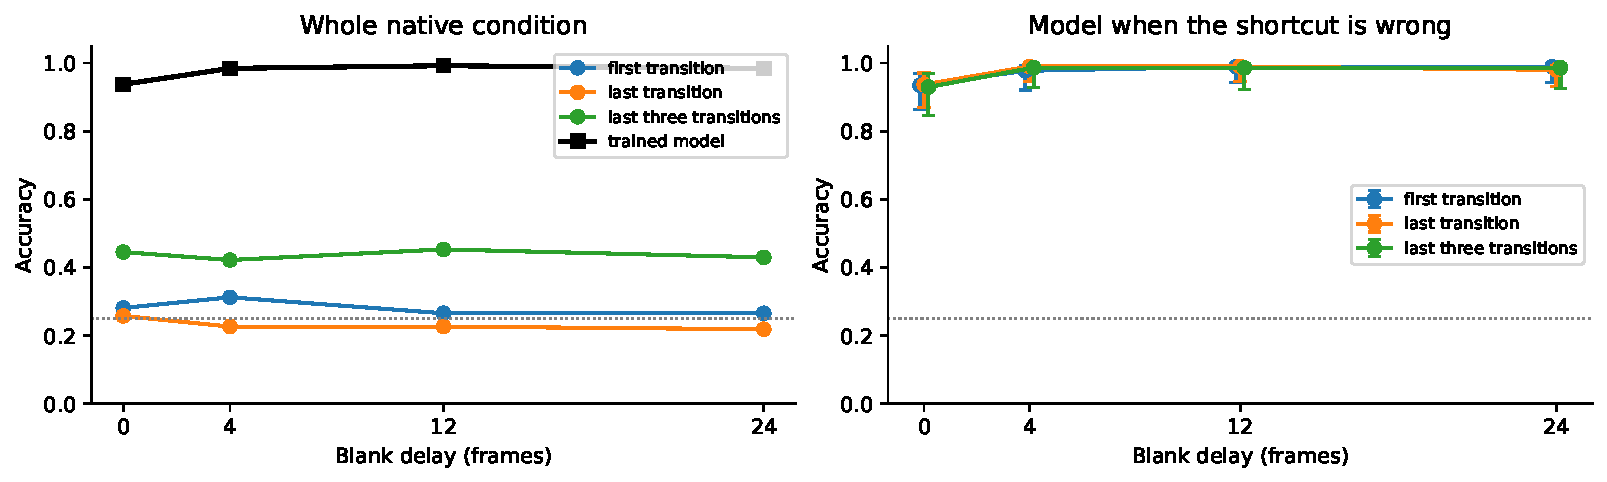
\includegraphics[width=.98\textwidth,height=.65\textheight,keepaspectratio]{../motion_duration_cued/figures/literature_temporal_shortcuts.pdf}
\captionof{figure}{Saved-trial temporal-strategy comparison. Left: trained-model and shortcut accuracies. Right: model accuracy restricted to trials where each shortcut is wrong. Error bars are within-condition Wilson intervals. Dotted line marks four-choice chance. The plotted delay affects retention after the same number of motion transitions.}
\end{minipage}\end{center}
\begingroup\small\renewcommand{\arraystretch}{.95}\begin{longtable}{rrlrrr}\toprule Delay & $n$ & Shortcut & Rule correct & Conflict $n$ & Model on conflict\\\midrule\endhead
0 & 128 & First & 28.1\% & 92 & 93.5\%\\
0 & 128 & Last three & 44.5\% & 71 & 93.0\%\\
0 & 128 & Last & 25.8\% & 95 & 93.7\%\\
4 & 128 & First & 31.2\% & 88 & 97.7\%\\
4 & 128 & Last three & 42.2\% & 74 & 98.6\%\\
4 & 128 & Last & 22.7\% & 99 & 99.0\%\\
12 & 128 & First & 26.6\% & 94 & 98.9\%\\
12 & 128 & Last three & 45.3\% & 70 & 98.6\%\\
12 & 128 & Last & 22.7\% & 99 & 99.0\%\\
24 & 128 & First & 26.6\% & 94 & 98.9\%\\
24 & 128 & Last three & 43.0\% & 73 & 98.6\%\\
24 & 128 & Last & 21.9\% & 100 & 98.0\%\\
\bottomrule\end{longtable}\endgroup
The model remains accurate when these short-history rules fail. This directly rejects the tested shortcut descriptions for these movies. It establishes use of a richer temporal summary; order-controlled evidence is the next test for distinguishing exact counts from other recurrent summaries.

\subsection{Agreement, difference and scientific interpretation}
The existing retention and attention interventions support selected temporal integration. The new shortcut comparison quantifies how much the behavior exceeds single-observation explanations. A full temporal-weighting account additionally requires count-matched sequences with systematically rearranged early and late evidence.

\subsection{The next discriminating experiment}
Keep direction counts fixed and reverse or permute their order. Then exchange early and late evidence while preserving the count margin. Fit temporal weights on held-out sequences and test whether a learned bound, leak or uniform count best predicts errors.

This last experiment is a proposed test; the results above are the completed frozen-model measurements.
\clearpage\section{Target selection and distractor rejection in cued motion-change detection}
\textbf{Scientific question.} Which moving signal is allowed to influence a covert change report?

The frozen checkpoint at update 204,289 achieved an equal-condition mean accuracy of 95.83\% across 3 native conditions (384 trials). The following comparisons use that same checkpoint and the measured interventions and population recordings in this paper.

\subsection{What the model measurements establish}
The target and foil interventions reveal a selection-dependent detector. Suppressing target priority reduces correct reports, and increasing foil priority also reduces performance. The baseline experiment provides little evidence for an additional benefit from foil suppression at the tested native signal strength. Spatial-memory disruption immediately before the change is especially costly, linking the event decision to the preceding cued state. Both global and comparison memories contain readable event information at the end of the trial. A pre-change comparison-memory reset tests dependence at that moment; subsequent visual comparisons remain available and can rebuild later evidence. Event-separated response curves distinguish missed relevant changes from inappropriate foil reports.

\subsection{Arcizet and Krauzlis (2018): macaque experiment}
Monkeys detected cued motion changes with a joystick while maintaining fixation. Caudate neurons encoded relevant location and task epoch, extending spatial-selection signals beyond overt orienting movements. \cite{bio_arcizet}

This is the closest task-family relation: maintain fixation, monitor cued motion and ignore an uncued event. The model’s spatial state can carry location and phase information, and its head reports a discrete event decision. Epoch and location decoders therefore parallel the questions asked of caudate activity. The model has a distributed recurrent implementation rather than an anatomically identified caudate circuit.

\subsection{Bollimunta, Bogadhi and Krauzlis (2018): macaque experiment}
Reversible FEF and SC inactivation impaired covert motion-change detection. Comparing the two interventions in a shared behavioral framework tested their contributions to selection during maintained fixation. \cite{bio_bollimunta}

Target suppression and foil enhancement impair the model’s detection, matching the functional importance of spatial selection. A logit dose changes normalized routing immediately and can alter later recurrent states. Biological inactivation changes a region’s activity and network interactions over a different spatial and temporal extent. The useful common comparison is the pattern of target hits, foil reports and catches under matched stimulus strength.

\subsection{Lovejoy and Krauzlis (2010): macaque experiment}
SC inactivation shifted motion judgments away from signals in the affected field toward competing information elsewhere. Deficits depended strongly on informative distractors; affecting the foil location favored judgments based on the cued signal. \cite{bio_lovejoy}

The animal result demonstrates competition-dependent use of motion evidence and a favorable shift when the foil is affected. Our native experiment shows little additional benefit from foil suppression at its tested strength. This is a substantive incomplete agreement: the model shows selection costs, while the predicted benefit from removing competition needs more favorable measurement conditions or a different computation.

\subsection{Theory and the model computation}
A shared-priority account says the decision depends on selected evidence, not simply on whether a visual change exists. Spatial memory retains the cue and prechange context; visual comparison provides event evidence; the readout must use the relevant location. Suppressing the target can remove useful evidence, and enhancing the foil can admit misleading evidence. The complementary improvement after foil suppression requires that the foil was limiting performance and that the remaining target evidence is usable. Native target changes here are relatively large, so a high baseline can hide an improvement. However, a ceiling explanation should be tested by lowering target strength, rather than assumed from the direction of attention redistribution.

\subsection{Agreement, difference and scientific interpretation}
The model agrees strongly with a causal selection requirement and with retained spatial context. It only partly reproduces the proposed reciprocal benefit-and-cost pattern. The next comparison should isolate informative competition, because that was central to the animal result and is more specific than a generic attention lesion.

\subsection{The next discriminating experiment}
Cross target strength with absent, uninformative and counterinformative foil events. Apply target and foil suppression separately, retain matched catches, and fit sensitivity and criterion. Predict a selective benefit of foil suppression only where foil information actually degrades the untreated decision.

This last experiment is a proposed test; the results above are the completed frozen-model measurements.
\clearpage\section{Retrospective selection of an orientation-location binding}
\textbf{Scientific question.} Can the observer retain which feature belonged where, then retrieve the relevant assignment after a cue?

The frozen checkpoint at update 204,289 achieved an equal-condition mean accuracy of 100.00\% across 4 native conditions (512 trials). The following comparisons use that same checkpoint and the measured interventions and population recordings in this paper.

\subsection{What the model measurements establish}
The all-location reconstruction provides a direct storage result: the original orientation inventory remains readable during the blank interval, before the retrospective cue identifies a target. Spatial-memory reconstruction is particularly strong. A mid-delay spatial reset and a later target-priority suppression each impair the final binding judgement, identifying storage and retrieval selection as separate causal stages. The final answer becomes explicit in global memory after the cue and probe supply the information needed to define it. The preserved inventory has native structure—four equally spaced orientations assigned to locations—so the result concerns retention of that structured array and its spatial assignment.

\subsection{Wheeler and Treisman (2002): human experiment}
Change-detection experiments separated memory for features from memory for their combinations. Binding was vulnerable to interference, motivating a distinction between retained feature information and attention-dependent integration. \cite{bio_wheeler}

Our probe can exchange orientations between locations while preserving the overall inventory. This directly tests assignment rather than the mere presence of features. Delay reconstruction shows the inventory is readable before the retrospective cue, while spatial reset and later target inhibition separately impair storage and retrieval. Those measurements make the binding interpretation more concrete than terminal accuracy alone.

\subsection{Bays, Catalao and Husain (2009): human experiment and theory}
Continuous-report errors reflected both feature and location memory. Accounting for their joint uncertainty supported a shared-resource description in which precision changes with the number of remembered objects. \cite{bio_bays}

A wrong-location report can reflect an assignment error even when feature content survives. Our binary swap decision compresses those possibilities into correct or incorrect. Reconstructing every location’s orientation permits a more informative error analysis: compare decoded angles with the true local angle and with the other stored angles. The equally spaced native inventory makes this especially important because it introduces predictable structure.

\subsection{Griffin and Nobre (2003): human experiment}
Cues presented before or after a visual array improved recognition of relevant locations. Behavioral and electrophysiological results linked orienting in perception and memory while revealing differences between precue and retrocue processing. \cite{bio_griffin}

The late cue selects an internal representation rather than a visible sample. The model’s before-cue reconstruction and after-cue attention sequence provide a natural parallel. A successful retrocue computation should first preserve several assignments, then prioritize the relevant one. Probe-period inhibition tests the second operation without erasing the original movie.

\subsection{Theory and the model computation}
Binding can be understood as retaining a joint relation between a location and a feature. Knowing all four orientations is insufficient if their positions are forgotten. A spatial recurrent field provides an explicit coordinate system for such relations, while global memory can later express whether the cued assignment changed. The current all-location reconstruction supports retained structured content; causal spatial disruption shows that this state matters. A resource account predicts gradual loss of precision or increasing assignment errors as load and similarity increase. The native task fixes a structured set of four orientations, so a load-dependent resource law must be tested with independent feature draws and additional set sizes.

\subsection{Agreement, difference and scientific interpretation}
The strongest agreement is the separation of retained content, spatial assignment and retrospective selection. The main protocol difference is the constrained orientation inventory. That structure can make inference easier than remembering arbitrary independent feature-location pairs and should be varied before interpreting native perfection as unlimited binding capacity.

\subsection{The next discriminating experiment}
Use independent orientations, then vary set size and minimum angular separation. Include feature substitutions and pure swaps. Measure local-angle precision, other-item confusions and binary behavior together, with delay and retrieval interventions separated in time.

This last experiment is a proposed test; the results above are the completed frozen-model measurements.
\clearpage\section{Recognition of an exact natural-image sample among intervening images}
\textbf{Scientific question.} Why does recognition remain good for repeats while novel images become increasingly likely to be accepted?

The frozen checkpoint at update 204,289 achieved an equal-condition mean accuracy of 94.27\% across 12 native conditions (1,536 trials). The following comparisons use that same checkpoint and the measured interventions and population recordings in this paper.

\subsection{What the model measurements establish}
Increasing the study load primarily increases false recognition of novel probes, while genuine repeats retain a high hit rate. This separates the dominant error pattern from simple disappearance of every stored image. The spatial-memory reset produces a large cost in the lower-load neural condition, and the final global state carries a strong recognition signal. The serial-position curves describe which stored items are most likely to be accepted; the last-image reconstruction describes only one component of the retained content. Together, these measures support studying familiarity accumulation and interference, alongside the precision with which individual study items can be recovered.

\subsection{Miller, Li and Desimone (1993): macaque experiment}
IT responses carried match-related information during delayed matching. Stimulus-selective delay activity could be disrupted by intervening stimuli, separating visible delay activity from successful later recognition. \cite{bio_miller93}

The model’s growing false-recognition rate with study load makes match-related population signals especially relevant. The biological result distinguishes a later recognition signal from uninterrupted activity for a sample. Our last-image reconstruction describes one retained item, while the recognition decision may depend on a broader aggregate of studied content. These are different readouts of memory.

\subsection{Miller, Erickson and Desimone (1996): macaque experiment}
A delayed matching task with intervening test objects examined prefrontal signals for remembered samples and matching decisions. It provided a comparison with temporal-cortex mechanisms under interference. \cite{bio_miller96}

Intervening images are a direct interference manipulation in both task families. The model must determine membership in a list, whereas delayed matching can designate one sample as the relevant item. That rule difference changes which intervening images should be stored or ignored. Comparing the same image sequence under sample-only and any-studied-item rules would reveal whether the network can protect a selected memory.

\subsection{Bays, Catalao and Husain (2009): human experiment and theory}
Continuous-report errors reflected both feature and location memory. Accounting for their joint uncertainty supported a shared-resource description in which precision changes with the number of remembered objects. \cite{bio_bays}

A distributed-resource account predicts declining precision as more content is retained. Recognition errors, however, also depend on the threshold for declaring a match. The signal-detection reanalysis below separates sensitivity from positive-response tendency across load. A high hit rate with rising false alarms can arise from overlapping familiarity distributions, a criterion shift, or both; accuracy alone does not decide among them.

\subsection{Theory and the model computation}
A familiarity-style computation compares the probe with an aggregate trace of previous images. As more images contribute, a novel probe can accidentally resemble some part of that trace. A more item-specific computation stores separable representations and compares the probe against each. The model’s spatial-reset cost establishes that retained state supports the judgment, while its high repeat acceptance and increasing novel acceptance identify a characteristic interference pattern. The added sensitivity-and-criterion table expresses that pattern in a common recognition framework. It uses finite-sample correction for perfect rates and keeps probe-hold conditions separate. An empty study list contains no genuine repeats, so sensitivity is undefined there even when correct rejection is perfect.

\subsection{Additional analysis prompted by the biological comparison}
The table re-expresses the existing native recognition decisions as repeat hits, novel-image false alarms, sensitivity and criterion. Positive means ``previously studied. Sensitivity is $d'=\Phi^{-1}(\widetilde H)-\Phi^{-1}(\widetilde F)$ and criterion is $c=-[\Phi^{-1}(\widetilde H)+\Phi^{-1}(\widetilde F)]/2$. Here $\Phi^{-1}$ converts a cumulative probability to a standard-normal quantile; $\widetilde H=(h+0.5)/(n_1+1)$ and $\widetilde F=(f+0.5)/(n_0+1)$ use counts of hits $h$, false alarms $f$, repeat opportunities $n_1$ and novel opportunities $n_0$. The correction keeps perfect observed rates finite. Negative criterion indicates a tendency toward positive reports in this descriptive signal-detection coordinate system.

\begin{center}\begin{minipage}{\textwidth}
\centering
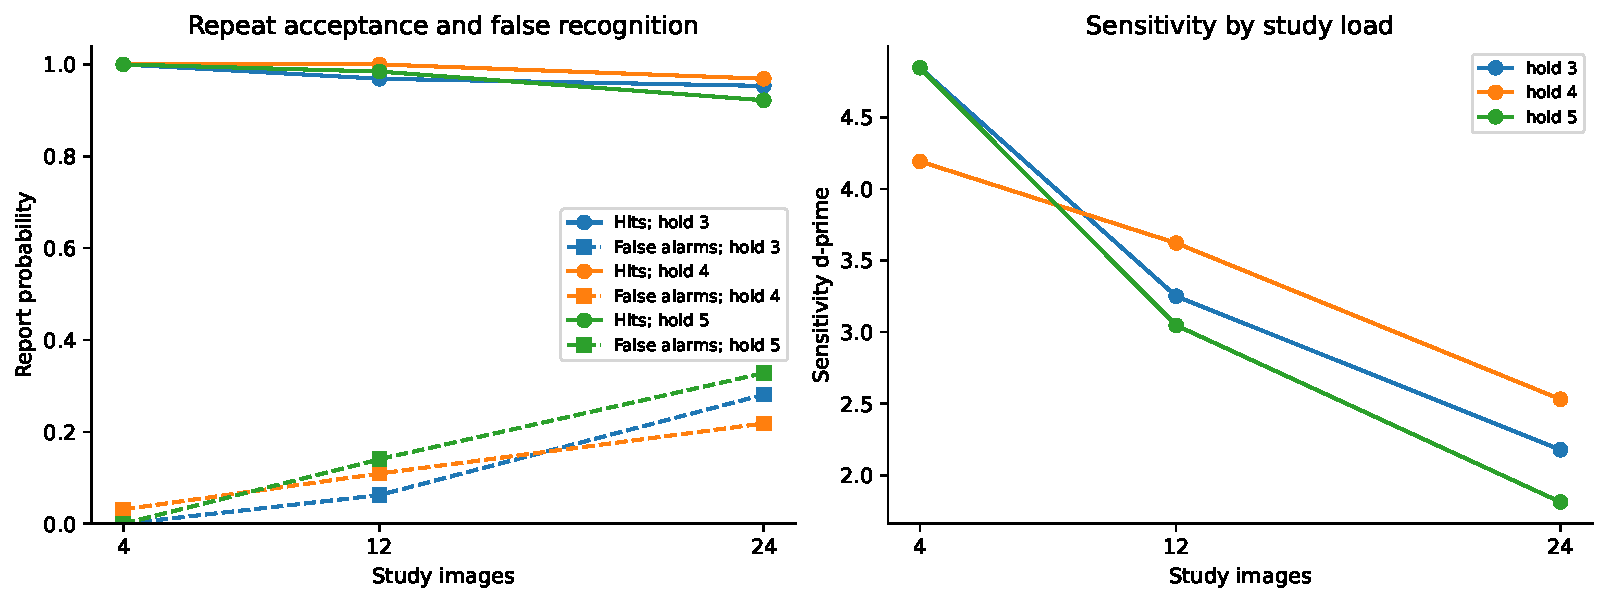
\includegraphics[width=.98\textwidth,height=.65\textheight,keepaspectratio]{../image_recognition/figures/literature_recognition_sdt.pdf}
\captionof{figure}{Recognition reanalysis of the saved native trials. Curves retain the three probe-hold conditions. Hits stay high while false recognition grows with study load; sensitivity generally decreases. These are descriptive condition estimates. There are 64 repeats and 64 novel probes per nonempty-list condition. Source-image clustering used elsewhere in the paper remains necessary for inferential comparisons across repeated photographs.}
\end{minipage}\end{center}
\begin{longtable}{rrrrrr}\toprule Load & Hold & Hits/repeats & False/novel & $d^{\prime}$ & $c$\\\midrule\endhead
0 & 3 & 0/0 & 0/128 & -- & --\\
0 & 4 & 0/0 & 0/128 & -- & --\\
0 & 5 & 0/0 & 0/128 & -- & --\\
4 & 3 & 64/64 & 0/64 & 4.85 & -0.00\\
4 & 4 & 64/64 & 2/64 & 4.19 & -0.33\\
4 & 5 & 64/64 & 0/64 & 4.85 & -0.00\\
12 & 3 & 62/64 & 4/64 & 3.25 & -0.14\\
12 & 4 & 64/64 & 7/64 & 3.62 & -0.61\\
12 & 5 & 63/64 & 9/64 & 3.05 & -0.47\\
24 & 3 & 61/64 & 18/64 & 2.18 & -0.52\\
24 & 4 & 62/64 & 14/64 & 2.53 & -0.50\\
24 & 5 & 59/64 & 21/64 & 1.81 & -0.47\\
\bottomrule\end{longtable}
The empty-list condition has no repeat opportunities, so sensitivity and criterion are undefined there. At higher loads, reduced sensitivity and a positive-report tendency coexist. A criterion-only explanation would fail to capture the observed decrease in separation under this convention; an item-similarity analysis can identify what makes the novel probes seem familiar.

\subsection{Agreement, difference and scientific interpretation}
The model agrees with interference-sensitive recognition and a population-level memory signal. It differs from a simple all-or-none forgetting account because errors are concentrated in accepting novel probes. The biological comparison becomes sharper by measuring image similarity and list membership separately rather than treating a single average recognition score as memory capacity.

\subsection{The next discriminating experiment}
Stratify novel probes by similarity to the study list and compare them with repeated items at different serial positions. Fit a held-out familiarity predictor and an itemwise nearest-memory predictor. Use matched images across list lengths to separate interference from differences in picture difficulty.

This last experiment is a proposed test; the results above are the completed frozen-model measurements.
\clearpage\section{Value-cued priority and causal competition in a four-location change task}
\textbf{Scientific question.} Does suppressing priority at a highly probable location harm detection there while helping a change elsewhere?

The frozen checkpoint at update 204,289 achieved an equal-condition mean accuracy of 67.97\% across 3 native conditions (384 trials). The following comparisons use that same checkpoint and the measured interventions and population recordings in this paper.

\subsection{What the model measurements establish}
The strong-change counterfactual reveals a pronounced cost of removing priority from the cued location and a large cost of increasing that priority when the change is elsewhere. Uncued detection is already high in the 18-degree sham condition. The exploratory two-, four- and eight-degree follow-up removes that ceiling, but still finds no uncued improvement under cue inhibition; at eight degrees, cued detection falls by about 29 percentage points while uncued detection is unchanged. Thus the requested combination of cued cost and uncued benefit is not recovered for this checkpoint in these experiments. Catch trials show how priority also changes positive-response tendency. Native performance at the smallest angle is substantially poorer than at larger angles, making a single pooled score an incomplete description. Because comparison memory remains zero throughout these seven frames, the measured competition is implemented by the shared visual-attention and recurrent pathways.

\subsection{Lovejoy and Krauzlis (2010): macaque experiment}
SC inactivation shifted motion judgments away from signals in the affected field toward competing information elsewhere. Deficits depended strongly on informative distractors; affecting the foil location favored judgments based on the cued signal. \cite{bio_lovejoy}

The biological experiment motivates testing both sides of competition. In VDA, a change anywhere receives a positive label; in the cued motion discrimination experiment, the instructed signal determines the correct direction. Our counterfactual bottom-right cue with a top-left change deliberately tests behavior outside the native 100-percent-validity contingency. It probes how strongly the cue governs the detector despite physically informative evidence elsewhere.

\subsection{Basso and Wurtz (1998): macaque experiment}
SC buildup activity varied with target probability, including when probability changed while the display remained fixed. More possible targets reduced preparatory activity, linking selection state with uncertainty and saccade latency. \cite{bio_basso}

Cue validity is a probability instruction. The SC study shows why probability should be manipulated independently of the visible array. Our condition-resolved maps can ask whether the same four Gabors receive different allocation under different displayed validity. The biological endpoint was saccade preparation, while our endpoint is a change report; both expose how expected relevance changes a spatial selection state.

\subsection{Zenon and Krauzlis (2012): macaque experiment}
SC inactivation impaired attentive behavior while established attentional modulation in visual cortex persisted. Behavioral selection and cortical response enhancement could therefore dissociate. \cite{bio_zenon}

The dissociation between cortical enhancement and behavior makes it important to inspect both the allocation map and the final report. In this model, the direct manipulation checks show that the intervention changes routing. A changed map alone does not imply improved use of the newly favored evidence. The weak-change follow-up supplies the corresponding behavioral test.

\subsection{Theory and the model computation}
The immediate softmax effect of inhibiting one region is mathematically guaranteed: the remaining regions receive a larger share of total attention. Behavioral improvement is a separate prediction. It requires useful change information to be represented, enough weight to reach it, and a readout that interprets it correctly. The strong-change sham already detects many uncued events. Lowering the angle to two, four and eight degrees removes that easy explanation for a missing benefit. At eight degrees, inhibition costs about 29 percentage points for cued events while uncued detection remains unchanged. The seven-frame trials keep the long-window comparison memory at zero, so these effects arise through the shared visual and recurrent pathways. This focuses the mechanism on routing, local temporal evidence and recurrent readout.

\subsection{Agreement, difference and scientific interpretation}
The model shows the cued impairment side of the proposed dual effect. It does not recover a reliable uncued improvement in the tested weak-change follow-up. This updates the earlier promising strong-signal interpretation: the evidence supports asymmetric behavioral consequences of redistribution, even though spatial competition itself is present.

\subsection{The next discriminating experiment}
Use one matched change-strength grid for cued, uncued and catch events, with independent cue-validity levels. Plot sensitivity and criterion alongside allocation. The crucial prediction is a positive uncued sensitivity change paired with a negative cued change, rather than merely more positive reports after inhibition.

This last experiment is a proposed test; the results above are the completed frozen-model measurements.
\clearpage\section{Priority competition and unexpected changes across nine visual locations}
\textbf{Scientific question.} How does cue-dependent competition scale when nine visual locations share the same spatial representation?

The frozen checkpoint at update 204,289 achieved an equal-condition mean accuracy of 68.49\% across 3 native conditions (384 trials). The following comparisons use that same checkpoint and the measured interventions and population recordings in this paper.

\subsection{What the model measurements establish}
The corner-to-corner counterfactual again shows a strong cued detection cost under cue inhibition. The uncued benefit at the strong signal is smaller and uncertain. The weak-change follow-up again produces a cued cost at eight degrees, about 35 percentage points, with no uncued benefit. It therefore does not recover the joint dual effect after correction across the three VDA follow-ups. Nine stimulus cells occupy unequal numbers of the ten-by-ten model sites, so the recorded mass and affected patch counts help interpret a common per-patch logit dose. Decodable change information increases across the visual-to-recurrent hierarchy, and spatial-memory reset impairs the native condition. The combined measurements connect spatial competition to retained sample information while separating local intervention geometry from behavioral sensitivity.

\subsection{Reynolds, Chelazzi and Desimone (1999): macaque experiment and theory}
For two stimuli within a receptive field, attention shifted the response toward that evoked by the attended item alone. The findings supported biased competition between simultaneously represented stimuli. \cite{bio_competition}

The animal experiment motivates comparing responses with and without competing stimuli while holding the target fixed. Our nine-cell array adds competitors but also changes the mapping from stimuli to the 10-by-10 model grid. Region mass must therefore be interpreted with the number of represented sites and their visual occupancy. A common logit dose can affect unequal amounts of evidence across cells.

\subsection{Basso and Wurtz (1998): macaque experiment}
SC buildup activity varied with target probability, including when probability changed while the display remained fixed. More possible targets reduced preparatory activity, linking selection state with uncertainty and saccade latency. \cite{bio_basso}

Probability-dependent selection is separable from the number of visible objects. VDA9 can exploit that distinction by keeping all nine cells present and varying only the cue information. The two native corner cue positions also permit matched spatial comparisons. The appropriate neural analogue is a change in preparatory selection for the same display, followed by an event-dependent report.

\subsection{Bollimunta, Bogadhi and Krauzlis (2018): macaque experiment}
Reversible FEF and SC inactivation impaired covert motion-change detection. Comparing the two interventions in a shared behavioral framework tested their contributions to selection during maintained fixation. \cite{bio_bollimunta}

The inactivation comparison motivates examining spatially specific detection costs under a fixed covert task. The model has a strong cued cost under inhibition, and weak eight-degree changes lose about 35 percentage points at the cue. The absence of an uncued gain indicates that restoring a larger relative share of attention elsewhere does not automatically restore a useful detector.

\subsection{Theory and the model computation}
Biased competition is a useful theory when several representations compete for a downstream effect. In the model, normalized spatial weights explicitly implement that competition, while recurrent memory supplies the previous visual state needed to detect change. The interpretation must include geometry: nine stimulus cells divide into a ten-site axis unevenly, and patch centers can sample different fractions of each cell. Increased set size can therefore alter feature quality, storage demand and selection competition together. The present spatial reset cost and improved recurrent answer decoding show that retained processing helps, but they do not assign all extra difficulty to an attentional capacity limit. The condition atlas and manipulation checks supply the needed map-level view before behavioral comparisons are pooled.

\subsection{Agreement, difference and scientific interpretation}
The agreement is cue-sensitive, memory-dependent competition with a reproducible cued suppression cost. The difference is the missing reciprocal improvement and the discrete grid’s unequal sampling. Both are scientifically useful: they specify which parts of the shared-selection account work and where stimulus quality or readout can limit its behavioral expression.

\subsection{The next discriminating experiment}
Render nine equally sampled apertures on a grid that gives each one the same number of model sites, and compare with the native resize. Hold target pixels fixed while adding distractors. A competition account predicts a distractor-dependent impairment beyond any change caused by target raster quality.

This last experiment is a proposed test; the results above are the completed frozen-model measurements.
\clearpage\section{Shared spatial priority under sixteen-location change competition}
\textbf{Scientific question.} Is poorer performance in a dense array caused by selection, representation, memory, or shared variability?

The frozen checkpoint at update 204,289 achieved an equal-condition mean accuracy of 64.84\% across 3 native conditions (384 trials). The following comparisons use that same checkpoint and the measured interventions and population recordings in this paper.

\subsection{What the model measurements establish}
The sixteen-location condition combines greater competition with a different sampling of each Gabor on the common grid. Its weaker native discrimination and the absence of a clear uncued gain in the strong-signal cue-inhibition experiment make it especially useful for separating attention redistribution from successful change extraction. Cue inhibition also changes catch performance, so the report criterion must be measured alongside hits. In the weaker-signal follow-up, cued costs at four and eight degrees survive the cross-VDA correction, while the uncued point estimates remain negative and do not show a reliable improvement. The requested dual effect is therefore absent at these tested strengths for this checkpoint. The recurrent populations contain more answer information than the early capacity-matched visual probes, and spatial-memory reset is harmful. These observations identify recurrent processing as useful even when the final detector remains imperfect.

\subsection{Cohen and Maunsell (2009): macaque experiment}
Population recordings in V4 during an orientation-change task linked much of the attentional improvement in population sensitivity to reduced shared variability, beyond changes in average firing rates. \cite{bio_cohen}

The biological result concerns trial-to-trial variability after controlling stimulus condition. Our frozen model is deterministic for an identical movie, so variability across randomly generated movies primarily reflects changing input. Correlations across those movies are signal-dependent correlations. To test the proposed neural mechanism, repeated identical stimuli would need an explicit internal-noise model and a separately defined residual covariance analysis.

\subsection{Reynolds, Chelazzi and Desimone (1999): macaque experiment and theory}
For two stimuli within a receptive field, attention shifted the response toward that evoked by the attended item alone. The findings supported biased competition between simultaneously represented stimuli. \cite{bio_competition}

Dense displays create a natural competition challenge. The present model’s priority intervention changes access to spatial representations, and its spatial reset harms detection. A target-alone versus target-with-competitors comparison would reveal whether the same target evidence degrades because of other items, independently of the smaller per-item raster in the native sixteen-cell condition.

\subsection{Zenon and Krauzlis (2012): macaque experiment}
SC inactivation impaired attentive behavior while established attentional modulation in visual cortex persisted. Behavioral selection and cortical response enhancement could therefore dissociate. \cite{bio_zenon}

A detector can fail even when a visual representation remains enhanced. Here, redistribution under cue inhibition is established, but weak four- and eight-degree experiments show reliable cued costs without an uncued gain. This is a useful model example of the gap between changing a selection signal and obtaining a behavioral improvement. The specific neural mechanism must be judged from representational and decision measurements together.

\subsection{Theory and the model computation}
Three bottlenecks can produce the same accuracy decline. A sensory bottleneck loses the small orientation change during rasterization or feature extraction. A memory bottleneck loses the relevant prechange orientation. A selection or readout bottleneck retains usable information but fails to compare the right location. The experiments already show recurrent information and a spatial-memory dependency, yet that does not exclude a sensory limitation at the smallest angles. The most direct next analysis would reconstruct prechange and postchange orientations at each cell and compare an external location-specific decoder with the agent’s binary response. Geometry and task load should be independently manipulated before attributing the VDA4-to-VDA16 difference to a single capacity parameter.

\subsection{Agreement, difference and scientific interpretation}
The model agrees with a causal role for recurrent spatial information and selective routing in dense change detection. It diverges from the hoped-for dual behavioral effect at the tested strengths. The data currently favor a multi-stage explanation of difficulty over a claim that attention redistribution alone is sufficient.

\subsection{The next discriminating experiment}
Cross item count with fixed item size and fixed retinal positions in a larger canvas. Decode local orientation differences, then repeat paired inhibition with matched catches. Introduce internal variability only as a separately documented model variant if testing residual-noise-correlation theories.

This last experiment is a proposed test; the results above are the completed frozen-model measurements.
\clearpage\section{Object memory, feature conjunctions and the selection of a matching location}
\textbf{Scientific question.} When remembered content is available, why does it sometimes fail to guide the choice of a matching object?

The frozen checkpoint at update 204,289 achieved an equal-condition mean accuracy of 53.11\% across 288 native conditions (36,864 trials). The following comparisons use that same checkpoint and the measured interventions and population recordings in this paper.

\subsection{What the model measurements establish}
The family-resolved results expose a selective failure that a task-wide average conceals. Distinct feature objects are matched almost perfectly, feature conjunctions remain substantially above chance, and irregular contour objects are much harder. The matched timing contrasts found no reliable rescue after correction across the tested timing comparisons. Full-resolution reconstruction provides a more specific explanation: spatial memory retains enough object information for an external pixel-distance matcher to achieve 95--100 percent accuracy in the two object conditions, whereas the agent makes much poorer choices on the same scenes. A follow-up also reconstructs the current candidates from local appearance features. Combining those decoded candidates with decoded spatial memory retains 100 percent accuracy for distinct objects and about 93 percent for similar objects, localizing a substantial deficit to the use of available representations. Joint decoding also improves distinct and similar fractals, although similar-fractal accuracy remains about 52 percent. Probe pairs are fitted separately within each stimulus condition, so these comparisons establish condition-specific information availability. Thus errors in using stored content and limitations of the stored or decoded representation coexist across stimulus families. The direct map check adds a second distinction: target stimulation raises final object-target allocation from about 21 percent to about 89 percent on the replay subset, while the full paired object experiments show only a partial behavioral rescue. Correct spatial allocation alone therefore does not restore successful object comparison. The changed-sample, identical-array experiment independently measures whether the agent uses its remembered sample to control choice and spatial allocation. Together, these measurements motivate a direct route from distributed spatial memory into the search computation, while identifying similar fractals as a separate demanding test of representational precision.

\subsection{Chelazzi, Miller, Duncan and Desimone (1993): macaque experiment}
Monkeys remembered a picture and selected its match from a small array. IT showed sample-related delay activity, followed during search by suppression of nontarget responses and dominance of the target representation. \cite{bio_chelazzi}

The basic sequence closely matches the model task: sample, delay, then an array containing the match. The animal result links remembered object content to later target selection. Our strongest comparison is the separation between retained information and its use. Irregular-object content can be reconstructed well enough for an external matcher to succeed, while the trained agent remains much poorer on the same scenes.

\subsection{Soto, Heinke, Humphreys and Blanco (2005): human experiment}
A remembered colored shape facilitated line search when it surrounded the target and impaired search when it surrounded a distractor. Effects extended to early responses and the first saccade. \cite{bio_soto}

Human memory can bias attention even when the remembered item is incidental to the current target. Our identical-array experiment changes only the preceding sample, giving a direct test of memory-dependent choice and allocation. A model could change its answer through downstream comparison while leaving its attention map similar; measuring both outcomes distinguishes guidance of selection from use of memory after selection.

\subsection{Bichot, Rossi and Desimone (2005): macaque experiment}
During free visual search, V4 responses favored objects sharing target features across the display. The experiment related feature-based parallel bias to selection during search among complex items. \cite{bio_bichot}

Feature-based selection can favor partial target matches before an object is finally identified. Our feature-family success and irregular-object weakness make that distinction useful. Plot allocation to candidates sharing individual features, then separately assess the unique conjunction match. The existing four-location output can express a correct choice even when the internal priority pattern distributes weight across several partial matches.

\subsection{Theory and the model computation}
Guided-search theory separates a representation of what is sought, a priority map that selects candidates, and the comparison that establishes a match. The present architecture retains detailed spatial memory but derives its global attention query from previous global memory. This creates a possible access bottleneck: stored object detail may remain readable externally without entering the query or nonlinear comparator in a useful form. The external decoded-memory plus decoded-candidate matcher performs near perfectly for distinct objects and very well for similar objects. Yet forcing attention toward the target yields only a partial rescue. Together, these observations locate a difficulty beyond simple loss of the sample or failure to raise target allocation. Similar fractals retain a lower external-matcher ceiling, adding a representational precision limit for that family. \cite{bio_wolfe}

\subsection{Agreement, difference and scientific interpretation}
The model agrees with successful memory-guided selection for feature-defined objects and a useful memory trace across families. It differs sharply from a uniform object-template account: rich stored information is not consistently converted into a correct match. This is a mechanistic failure worth emphasizing rather than averaging away in the task-wide score.

\subsection{The next discriminating experiment}
Compare memory-to-query access, candidate encoding and the final comparator using matched scenes and independently fitted probes. A direct spatial-memory query route predicts larger improvements for irregular objects than for already-solved feature stimuli. Evaluate that prediction on the separate fresh-architecture experiment, with the present frozen model retained as the baseline.

This last experiment is a proposed test; the results above are the completed frozen-model measurements.
\clearpage\section{Feature contrast, exposure time and location reports in pop-out search}
\textbf{Scientific question.} How does a physically distinctive item become a selected location over successive processing steps?

The frozen checkpoint at update 204,289 achieved an equal-condition mean accuracy of 86.36\% across 24 native conditions (3,072 trials). The following comparisons use that same checkpoint and the measured interventions and population recordings in this paper.

\subsection{What the model measurements establish}
Additional processing of the same static array produces a large behavioral benefit. At the smallest color difference, accuracy rises from about 48 percent after one array frame to 100 percent after two. At a five-degree orientation difference it rises from 25 percent to about 83 percent after two frames, reaching about 86 percent after eight. The matched one-versus-eight-frame comparisons survive correction in five of the six feature-difference groups; the largest color difference is already at ceiling. Thus a physically available singleton is not necessarily converted into a correct location report on the first processing step. Repeated frames permit both recurrent state updates and re-evaluation of the visual pathways. The priority and state interventions then ask which parts of that processing support selection. Since item count is fixed at four, these curves characterize feature discrimination and temporal processing within that array size.

\subsection{Schall and Hanes (1993): macaque experiment}
Initial FEF visual responses did not distinguish target from distractor. Activity subsequently evolved to identify the target before the eye movement, separating stimulus onset responses from selection. \cite{bio_schall}

The animal experiment separates an initial visual response from later target selection. Our repeated static array likewise produces a large one-to-two-frame improvement for weak singletons. This is a functional parallel in the emergence of selection. The network’s frames are computation steps, so the comparison should concern ordering of processes and feature difficulty before assigning a biological time scale.

\subsection{Bichot, Rossi and Desimone (2005): macaque experiment}
During free visual search, V4 responses favored objects sharing target features across the display. The experiment related feature-based parallel bias to selection during search among complex items. \cite{bio_bichot}

Parallel feature bias and later selection can coexist. In the model, all sites are represented each frame and one normalized priority distribution weights their contribution. A later correct location report therefore need not imply serial inspection of every item. The time course of target-minus-distractor allocation and local feature evidence can reveal whether an early distributed signal becomes a concentrated selection.

\subsection{Ling, Liu and Carrasco (2009): human experiment and theory}
External-noise motion experiments separated spatial from feature-based attention. Threshold-versus-noise functions supported different combinations of population gain and tuning, giving behavioral tests of attentional mechanisms. \cite{bio_ling}

External-noise methods provide a way to separate weak feature evidence from poor selection. A small singleton difference can produce a subtle signal even when the display contains only four objects. Varying orientation noise around the distractor mean, separately from the target difference, would reveal whether extra model frames increase effective gain or improve exclusion of irrelevant feature variation.

\subsection{Theory and the model computation}
A priority-map account combines local distinctiveness with task-relevant feature information. Repeated frames allow the same static evidence to update recurrent state and feed back into the next selection step. In the present data, the weakest color singleton rises from roughly 48 percent after one frame to perfect performance after two; a five-degree orientation singleton rises from chance to about 83 percent. These are large processing-time effects despite an unchanged visible array. Guided Search supplies a framework in which selection and identification unfold over time, while the model provides an explicit recurrent implementation. To test classical search efficiency, however, item count must vary: fixed four-item trials measure processing duration and feature separation, not a reaction-time slope per added distractor. \cite{bio_wolfe}

\subsection{Agreement, difference and scientific interpretation}
The agreement is a time-dependent transition from visible feature information to useful target selection, especially for weak differences. The model’s discrete forced report and fixed set size differ from free-viewing or variable-size search experiments. These differences specify the next tests rather than weakening the observed temporal benefit.

\subsection{The next discriminating experiment}
Vary set size while holding item size, spacing and feature difference fixed. Record confidence crossing, final choice and target allocation. Compare target-present and target-absent trials, and test whether additional distractors affect identification time after controlling the singleton’s local contrast.

This last experiment is a proposed test; the results above are the completed frozen-model measurements.
\clearpage\section{Remembered motion as a template for selection among moving alternatives}
\textbf{Scientific question.} How can a remembered motion direction guide selection of a new moving pattern at a new location?

The frozen checkpoint at update 204,289 achieved an equal-condition mean accuracy of 97.74\% across 81 native conditions (10,368 trials). The following comparisons use that same checkpoint and the measured interventions and population recordings in this paper.

\subsection{What the model measurements establish}
Across 81 native conditions, mean accuracy is about 97.7 percent. The paired timing contrasts show no corrected benefit from extending the tested sample or array durations, consistent with high performance at the shorter settings. The sample and search candidates use independent dot layouts, so the task requires a motion template that survives a change in visual realization. At the middle delay, a capacity-matched linear decoder reconstructs the remembered direction with R-squared about 0.76 from global memory and 0.87 from spatial memory. Resetting global memory there reduces accuracy by about 73 percentage points in both selected direction-spacing conditions, whereas the spatial reset is less damaging. Target-priority inhibition during search separately costs about 70 to 90 percentage points. This combination identifies readable retained content, strong dependence on global memory, and a causal selection requirement in a successful search computation. Continuous direction reconstruction tests retention of that template, while the final location decoder tests its use after the candidates appear. Matched timing effects separate sample evidence from search evidence and intervening retention. The identical-array query switch provides a direct causal test of template dependence: only the preceding sample direction changes. Comparing its behavioral probability contrast with its attention contrast reveals whether memory influences spatial selection, the downstream decision, or both.

\subsection{Zaksas and Pasternak (2006): macaque experiment}
Monkeys compared two motion directions across a delay. MT and PFC carried direction information with transient delay signals; test responses depended on the remembered sample and related to the eventual decision. \cite{bio_zaksas}

The shared computation is retaining direction across a delay and comparing later motion with that content. Our independent sample and candidate dot layouts force transfer beyond the same dot arrangement. Mid-delay direction decoding and the large global-reset cost provide complementary evidence for a retained motion template. The biological task compared successive directions, whereas ours must choose among simultaneous locations.

\subsection{Chelazzi, Miller, Duncan and Desimone (1993): macaque experiment}
Monkeys remembered a picture and selected its match from a small array. IT showed sample-related delay activity, followed during search by suppression of nontarget responses and dominance of the target representation. \cite{bio_chelazzi}

The visual-search structure adds selection among candidates to memory comparison. Here the template is motion rather than a complex static picture. The strong performance across direction-spacing and timing conditions shows that this architecture can use one kind of remembered content to guide a location decision, even while irregular static-object search remains difficult.

\subsection{Ling, Liu and Carrasco (2009): human experiment and theory}
External-noise motion experiments separated spatial from feature-based attention. Threshold-versus-noise functions supported different combinations of population gain and tuning, giving behavioral tests of attentional mechanisms. \cite{bio_ling}

Feature-based motion attention offers a bridge from remembered direction to distributed selection. Candidate directions close to the remembered sample should produce more competition than distant ones. Measuring target and neighbor allocation as a function of angular separation would connect the template’s precision to spatial selection, while an external-noise manipulation would distinguish tuning precision from simple gain.

\subsection{Theory and the model computation}
A circular template can represent direction through its sine and cosine, allowing similarity to depend on angular distance rather than an arbitrary numeric label. The model need not use exactly this two-coordinate code; it can retain a distributed representation with the same geometry. At the middle delay, external direction reconstruction explains substantial variance in both global and spatial states. Resetting global memory produces a much larger behavioral cost than the spatial reset at that moment, identifying a particularly important carrier for subsequent matching. During search, target inhibition creates a separate major cost. These observations link content retention and spatial selection in a successful computation, rather than relying solely on a final correct answer. \cite{bio_wolfe}

\subsection{Agreement, difference and scientific interpretation}
The model agrees with an abstract motion memory that transfers across dot realizations and supports later selection. Its success contrasts with static object search and argues against a single universal failure of memory or attention. The likely difference concerns how each content type is encoded and made accessible to the query and comparison stages.

\subsection{The next discriminating experiment}
Match motion and static search for candidate similarity and baseline difficulty. Compare sample-switch effects on allocation, memory-to-query decodability and paired state interventions. Test whether adding uncertainty to motion templates recreates the static-search pattern of retained information with poor use.

This last experiment is a proposed test; the results above are the completed frozen-model measurements.
\clearpage\section{Source access and reproducibility}
The source ledger contains bibliographic metadata, a concise finding and the level of primary-source access used. Task chapters and their references are generated from neuroscience\_content.py and literature\_sources.py. New diagnostic tables and plots are reproduced by literature\_analysis.py from the saved native trials. Their input hashes are recorded in literature\_reanalysis\_provenance.json. Full native-trial and checkpoint provenance remains in the accompanying analysis package.
\begin{thebibliography}{99}
\bibitem{bio_competition} Reynolds, Chelazzi and Desimone (1999). Competitive mechanisms subserve attention in macaque areas V2 and V4. \href{https://pubmed.ncbi.nlm.nih.gov/10024360/}{Primary source}.
\bibitem{bio_normalization} Reynolds and Heeger (2009). The normalization model of attention. \href{https://pmc.ncbi.nlm.nih.gov/articles/PMC2752446/}{Primary source}.
\bibitem{bio_stokes} Stokes and colleagues (2013). Dynamic coding for cognitive control in prefrontal cortex. \href{https://pmc.ncbi.nlm.nih.gov/articles/PMC3898895/}{Primary source}.
\bibitem{bio_britten} Britten, Shadlen, Newsome and Movshon (1992). The analysis of visual motion: a comparison of neuronal and psychophysical performance. \href{https://pubmed.ncbi.nlm.nih.gov/1464765/}{Primary source}.
\bibitem{bio_salzman} Salzman, Britten and Newsome (1990). Cortical microstimulation influences perceptual judgements of motion direction. \href{https://pubmed.ncbi.nlm.nih.gov/2366872/}{Primary source}.
\bibitem{bio_ling} Ling, Liu and Carrasco (2009). How spatial and feature-based attention affect the gain and tuning of population responses. \href{https://pmc.ncbi.nlm.nih.gov/articles/PMC2696585/}{Primary source}.
\bibitem{bio_devalois_o} De Valois, Yund and Hepler (1982). The orientation and direction selectivity of cells in macaque visual cortex. \href{https://pubmed.ncbi.nlm.nih.gov/7112953/}{Primary source}.
\bibitem{bio_harrison} Harrison and Tong (2009). Decoding reveals the contents of visual working memory in early visual areas. \href{https://pubmed.ncbi.nlm.nih.gov/19225460/}{Primary source}.
\bibitem{bio_mcadams} McAdams and Maunsell (1999). Effects of attention on orientation-tuning functions of single neurons in macaque cortical area V4. \href{https://pubmed.ncbi.nlm.nih.gov/9870971/}{Primary source}.
\bibitem{bio_legge} Legge and Foley (1980). Contrast masking in human vision. \href{https://pubmed.ncbi.nlm.nih.gov/7463185/}{Primary source}.
\bibitem{bio_reynolds00} Reynolds, Pasternak and Desimone (2000). Attention increases sensitivity of V4 neurons. \href{https://pubmed.ncbi.nlm.nih.gov/10896165/}{Primary source}.
\bibitem{bio_campbell} Campbell and Robson (1968). Application of Fourier analysis to the visibility of gratings. \href{https://doi.org/10.1113/jphysiol.1968.sp008574}{Primary source}.
\bibitem{bio_devalois_f} De Valois, Albrecht and Thorell (1982). Spatial frequency selectivity of cells in macaque visual cortex. \href{https://pubmed.ncbi.nlm.nih.gov/7112954/}{Primary source}.
\bibitem{bio_regan} Regan and Beverley (1983). Spatial-frequency discrimination and detection: comparison of postadaptation thresholds. \href{https://pubmed.ncbi.nlm.nih.gov/6663371/}{Primary source}.
\bibitem{bio_derrington} Derrington, Krauskopf and Lennie (1984). Chromatic mechanisms in lateral geniculate nucleus of macaque. \href{https://pubmed.ncbi.nlm.nih.gov/6512691/}{Primary source}.
\bibitem{bio_lennie} Lennie, Krauskopf and Sclar (1990). Chromatic mechanisms in striate cortex of macaque. \href{https://pubmed.ncbi.nlm.nih.gov/2303866/}{Primary source}.
\bibitem{bio_flanagan} Flanagan, Cavanagh and Favreau (1990). Independent orientation-selective mechanisms for the cardinal directions of colour space. \href{https://pubmed.ncbi.nlm.nih.gov/2378069/}{Primary source}.
\bibitem{bio_field} Field, Hayes and Hess (1993). Contour integration by the human visual system: evidence for a local association field. \href{https://pubmed.ncbi.nlm.nih.gov/8447091/}{Primary source}.
\bibitem{bio_kapadia} Kapadia, Ito, Gilbert and Westheimer (1995). Improvement in visual sensitivity by changes in local context: parallel studies in human observers and in V1 of alert monkeys. \href{https://pubmed.ncbi.nlm.nih.gov/7576633/}{Primary source}.
\bibitem{bio_li} Li, Piech and Gilbert (2006). Contour saliency in primary visual cortex. \href{https://pubmed.ncbi.nlm.nih.gov/16772175/}{Primary source}.
\bibitem{bio_tolhurst97} Tolhurst and Tadmor (1997). Discrimination of changes in the slopes of the amplitude spectra of natural images: band-limited contrast and psychometric functions. \href{https://pubmed.ncbi.nlm.nih.gov/9509160/}{Primary source}.
\bibitem{bio_tolhurst00} Tolhurst and Tadmor (2000). Discrimination of spectrally blended natural images: optimisation of the human visual system for encoding natural images. \href{https://pubmed.ncbi.nlm.nih.gov/11144821/}{Primary source}.
\bibitem{bio_olshausen} Olshausen and Field (1996). Emergence of simple-cell receptive field properties by learning a sparse code for natural images. \href{https://www.nature.com/articles/381607a0}{Primary source}.
\bibitem{bio_griffin} Griffin and Nobre (2003). Orienting attention to locations in internal representations. \href{https://pubmed.ncbi.nlm.nih.gov/14709235/}{Primary source}.
\bibitem{bio_kiani} Kiani, Hanks and Shadlen (2008). Bounded integration in parietal cortex underlies decisions even when viewing duration is dictated by the environment. \href{https://pmc.ncbi.nlm.nih.gov/articles/PMC6670720/}{Primary source}.
\bibitem{bio_stine} Stine, Zylberberg, Ditterich and Shadlen (2020). Differentiating between integration and non-integration strategies in perceptual decision making. \href{https://pubmed.ncbi.nlm.nih.gov/32338595/}{Primary source}.
\bibitem{bio_mante} Mante, Sussillo, Shenoy and Newsome (2013). Context-dependent computation by recurrent dynamics in prefrontal cortex. \href{https://pubmed.ncbi.nlm.nih.gov/24201281/}{Primary source}.
\bibitem{bio_arcizet} Arcizet and Krauzlis (2018). Covert spatial selection in primate basal ganglia. \href{https://journals.plos.org/plosbiology/article?id=10.1371/journal.pbio.2005930}{Primary source}.
\bibitem{bio_bollimunta} Bollimunta, Bogadhi and Krauzlis (2018). Comparing frontal eye field and superior colliculus contributions to covert spatial attention. \href{https://pmc.ncbi.nlm.nih.gov/articles/PMC6120922/}{Primary source}.
\bibitem{bio_lovejoy} Lovejoy and Krauzlis (2010). Inactivation of primate superior colliculus impairs covert selection of signals for perceptual judgments. \href{https://pubmed.ncbi.nlm.nih.gov/20023651/}{Primary source}.
\bibitem{bio_wheeler} Wheeler and Treisman (2002). Binding in short-term visual memory. \href{https://pubmed.ncbi.nlm.nih.gov/11900102/}{Primary source}.
\bibitem{bio_bays} Bays, Catalao and Husain (2009). The precision of visual working memory is set by allocation of a shared resource. \href{https://pubmed.ncbi.nlm.nih.gov/19810788/}{Primary source}.
\bibitem{bio_miller93} Miller, Li and Desimone (1993). Activity of neurons in anterior inferior temporal cortex during a short-term memory task. \href{https://pubmed.ncbi.nlm.nih.gov/8463829/}{Primary source}.
\bibitem{bio_miller96} Miller, Erickson and Desimone (1996). Neural mechanisms of visual working memory in prefrontal cortex of the macaque. \href{https://pmc.ncbi.nlm.nih.gov/articles/PMC6579322/}{Primary source}.
\bibitem{bio_basso} Basso and Wurtz (1998). Modulation of neuronal activity in superior colliculus by changes in target probability. \href{https://pubmed.ncbi.nlm.nih.gov/9736670/}{Primary source}.
\bibitem{bio_zenon} Zenon and Krauzlis (2012). Attention deficits without cortical neuronal deficits. \href{https://pubmed.ncbi.nlm.nih.gov/22972195/}{Primary source}.
\bibitem{bio_cohen} Cohen and Maunsell (2009). Attention improves performance primarily by reducing interneuronal correlations. \href{https://pubmed.ncbi.nlm.nih.gov/19915566/}{Primary source}.
\bibitem{bio_chelazzi} Chelazzi, Miller, Duncan and Desimone (1993). A neural basis for visual search in inferior temporal cortex. \href{https://pubmed.ncbi.nlm.nih.gov/8497317/}{Primary source}.
\bibitem{bio_soto} Soto, Heinke, Humphreys and Blanco (2005). Early, involuntary top-down guidance of attention from working memory. \href{https://www.comp-psych.bham.ac.uk/publications/soto_jep2005.pdf}{Primary source}.
\bibitem{bio_bichot} Bichot, Rossi and Desimone (2005). Parallel and serial neural mechanisms for visual search in macaque area V4. \href{https://doi.org/10.1126/science.1109676}{Primary source}.
\bibitem{bio_wolfe} Wolfe (2021). Guided Search 6.0: An updated model of visual search. \href{https://doi.org/10.3758/s13423-020-01859-9}{Primary source}.
\bibitem{bio_schall} Schall and Hanes (1993). Neural basis of saccade target selection in frontal eye field during visual search. \href{https://pubmed.ncbi.nlm.nih.gov/8247155/}{Primary source}.
\bibitem{bio_zaksas} Zaksas and Pasternak (2006). Directional signals in the prefrontal cortex and in area MT during a working memory for visual motion task. \href{https://pubmed.ncbi.nlm.nih.gov/17093094/}{Primary source}.
\end{thebibliography}\end{document}